\chapter{相关器与事件表数据分析}
\label{chap:e14}

\begin{chapteropening}
上一章（第 \ref{chap:e13} 章）里，望远镜把每一个光子候选写成了一行记录：什么时候到、来自哪个站点、走哪个探测器通道、什么波长、什么偏振。一夜下来，这样的记录可能有几十亿行——它们静静地躺在磁盘上，本身既不是角直径，也不是 \(g^{(2)}\)，只是一堆时间戳。

本章要回答的，正是横在"一堆事件"和"一条可信曲线"之间的那道工序：怎样把这几十亿个时间戳，变成一条带误差棒、能复现、能拿去拟合物理模型的 \(|V|^2\) 或 \(g^{(2)}\)？我们会沿着一条主线走：先把事件表翻译成概率模型（写出似然），再定义相关估计量并做归一化，然后解决"算得完吗"（相关器的计算量标度），最后是全书数据分析里最容易被低估的一环——误差从哪来、为什么系统误差往往才是天花板。第 \ref{chap:e08} 章给过的延迟直方图、第 \ref{chap:e12} 章给过的 Fisher 语言，会在这里被真正用起来。
\end{chapteropening}

\section{从事件表到概率模型}
\label{sec:e14-model}

先约定记号。把一份标定后的事件表整体记作一个数据集
\begin{equation}
  \mathcal{D}
  =
  \left\{
  t_q,\ a_q,\ d_q,\ c_q,\ p_q,\ w_q,\ f_q
  \right\}_{q=1}^{N_{\rm evt}} ,
  \label{eq:e14-data}
\end{equation}
\begin{formulaexplain}
\(\mathcal D\) 是整张标定事件表；每个事件 \(q\) 带时间 \(t_q\)、站点 \(a_q\)、探测器 \(d_q\)、谱道 \(c_q\)、偏振 \(p_q\)、权重 \(w_q\) 和质量标记 \(f_q\)；\(N_{\rm evt}\) 是总事件数。它是后面一切估计量的原始"食材"。
\end{formulaexplain}
这里 \(t_q\) 是统一时间尺度上的到达时刻（单位 s，典型精度可达纳秒甚至几十皮秒），\(a_q,d_q,c_q,p_q\) 都是整数通道编号（无量纲），\(w_q\) 是权重（无量纲），\(f_q\) 是标记这条事件是否"干净"的质量位。这些字段怎么来、时钟怎么校、格式怎么定，是上一章（第 \ref{chap:e13} 章）的内容；这一章直接从"表已经在手上"开始。

分析的第一步不是画图，而是写下一个\textbf{选择函数}（selection function），它决定哪些事件参与后续计算：
\begin{equation}
  S_q = S(t_q,a_q,d_q,c_q,p_q,f_q),
  \qquad
  S_q\in\{0,1\}\ \text{或}\ [0,1] .
  \label{eq:e14-selection}
\end{equation}
\begin{formulaexplain}
\(S_q\) 是第 \(q\) 个事件的选择/权重；取 0 或 1 表示剔除或保留，取 \([0,1]\) 的连续值表示曝光、死时间、背景或效率带来的加权。它把"人为选点"变成一条能重跑的规则。
\end{formulaexplain}
为什么要如此正式？想象一个通道事件率是 \(10^{6}\,\mathrm{s^{-1}}\)，一小时观测就是 \(3.6\times10^{9}\) 个事件。谁也没法"看着图手动删几个坏点"——那既做不到，也不可复现。选择函数必须能由元数据（云量、PMT 电流、死时间标记、阈值）自动重新生成，这样光变、相关、拟合三层用的都是同一套口径。第 \ref{chap:e15} 章做误差预算时会反复强调：一切系统检验都要在同一套 \(S_q\) 下进行。

\paragraph{未分箱数据：非齐次泊松点过程}

事件在时间轴上是一个个离散的点，最自然的模型是\textbf{非齐次泊松点过程}（inhomogeneous Poisson point process）：某时刻、某通道的瞬时事件率是 \(\lambda(t,\bm{x}\mid\bm{\theta})\)，其中 \(\bm x\) 打包了通道、波长、偏振、天空位置等标签，\(\bm\theta\) 是我们最终想估计的物理参数。第 \ref{chap:e03} 章讲过：泊松过程里"很短一段时间内出现一个事件"的概率正比于率乘以时长，而且互不影响。我们就用这一点把似然一步步搭出来。

把整段观测切成许多极窄的小格 \(\Delta t\)，窄到每格里至多一个事件。第 \(i\) 格里"有一个事件"的概率约为 \(\lambda_i E_i\,\Delta t\)（\(E_i\) 是这一格的有效曝光），"没有事件"的概率约为 \(1-\lambda_i E_i\,\Delta t\approx e^{-\lambda_i E_i\Delta t}\)。整段观测的似然就是所有格子的连乘：占据的格子贡献 \(\lambda E\Delta t\)，空格子贡献 \(e^{-\lambda E\Delta t}\)。取对数：
\[
  \ln L
  =\sum_{q:\,S_q>0}\ln\!\big(\lambda(t_q,\bm x_q)\,E_q\,\Delta t\big)
   -\sum_{\text{所有格}}\lambda_i E_i\,\Delta t .
\]
让 \(\Delta t\to0\)：第一项里的 \(\ln\!\big(\lambda E_q\,\Delta t\big)=\ln\lambda+\ln E_q+\ln\Delta t\) 可以拆开，其中 \(\ln\Delta t\) 是分箱宽度、\(\ln E_q\) 是这一格的仪器/曝光项，二者都与待估参数 \(\bm\theta\) 无关，拟合时作为常数一起丢掉（注意曝光 \(E\) 本身并没有消失，它仍完整保留在第二项的积分里），故第一项只剩 \(\ln\lambda\)；第二个求和变成积分。于是
\begin{equation}
  \ln L(\bm\theta)
  =
  \sum_{q:\,S_q>0}\ln\lambda(t_q,\bm x_q\mid\bm\theta)
  -\int_{\mathcal T}\lambda(t,\bm x\mid\bm\theta)\,E(t,\bm x)\,dt\,d\bm x .
  \label{eq:e14-point-likelihood}
\end{equation}
\begin{formulaexplain}
\(\ln L\) 是点过程对数似然。第一项在每个真实事件处给模型率打分：事件落在高率区就加分。第二项是模型在有效曝光 \(E\) 上预言的总事件数：模型不能只在事件处冒尖，还得解释别处为什么没事件。
\end{formulaexplain}
逐个符号说清楚：\(\lambda\) 的单位是 \(\mathrm{s^{-1}}\)（或 \(\mathrm{s^{-1}\,channel^{-1}}\)），\(E(t,\bm x)\) 无量纲或带面积/效率因子，装的是坏天气、死时间、通道开关、滤光片透过率、观测窗口这些真实损耗。这条式子最重要的教学点是它的"平衡"：只让率在事件处高是骗不过第二项的，因为第二项会因预言太多事件而扣分。这正是天文学里的 Cash 统计量（Cash statistic），低计数时不能用对称的 \(\sqrt N\) 误差蒙混过去 \citep{1979ApJ...228..939C,1986ApJ...303..336G}。

\begin{figure}[tbp]
\centering
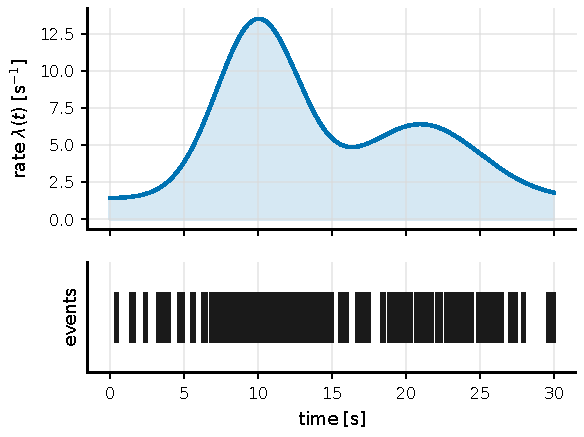
\includegraphics[width=0.72\linewidth]{figures/generated/chapter_07/ch07_poisson_likelihood.pdf}
\caption{非齐次泊松过程的画面。上图是随时间起伏的瞬时率 \(\lambda(t)\)，下图是由这个率随机"落下"的一串事件。似然式 \eqref{eq:e14-point-likelihood} 同时用到"事件落在高率处"和"整段积分率"两条信息；若只把事件重新分箱成一条光变曲线，就会丢掉一部分时间信息，快变或曝光不均时尤其明显。}
\label{fig:e14-poisson}
\end{figure}

\paragraph{分箱数据：退化成逐格泊松}

如果我们先把事件分进时间格、谱道或延迟格，点过程似然就退化成人人熟悉的\textbf{分箱泊松似然}。第 \(i\) 格观测到 \(d_i\) 个事件、模型预言 \(m_i(\bm\theta)\) 个，泊松概率是 \(P(d_i)=e^{-m_i}m_i^{d_i}/d_i!\)（见第 \ref{chap:e03} 章）。各格独立，取对数再求和：
\begin{equation}
  \ln L
  =\sum_i\Big[\,d_i\ln m_i(\bm\theta)-m_i(\bm\theta)-\ln(d_i!)\,\Big] .
  \label{eq:e14-binned-poisson}
\end{equation}
\begin{formulaexplain}
\(d_i\) 是第 \(i\) 格的观测计数，\(m_i\) 是模型计数，二者都无量纲。这是光变曲线、谱道、延迟直方图都能用的似然；它天生保留低计数时的不对称统计，不假装误差是高斯的。
\end{formulaexplain}
当某格计数 \(d_i\gtrsim20\) 且模型不贴边界时，泊松可近似成高斯，误差棒近似 \(\sqrt{d_i}\)；但当格子计数只有几个（延迟直方图的信号窗口常如此），就必须留在式 \eqref{eq:e14-binned-poisson}。还有一个坑要提前说：当模型里新增一个"强度必须非负"的分量（例如"有没有相关峰"），零强度落在参数边界上，似然比检验不再服从名义 \(\chi^2\) 分布，显著性得靠模拟或后验预测检验来标定 \citep{2002ApJ...571..545P}。对慢变背景和爆发筛选，Bayesian Blocks 会把时间轴自适应地切成若干"常率段"，数据空隙通过有效曝光（live time）进入而不被误认作"无事件" \citep{2013ApJ...764..167S}；但最终物理参数仍应回到明确的似然。

\section{两路事件如何长出相关峰}
\label{sec:e14-corr}

强度干涉的核心动作，是比较两个站点 \(a,b\) 的事件到达时间。第 \ref{chap:e08} 章已经从 \(g^{(2)}\) 得到过延迟直方图的思想；这里把它落成能对真实事件表运行的估计量。

第一步是算\textbf{校正后的时间差}。原始时间差里混着几何延迟和仪器延迟，必须先扣掉：
\begin{equation}
  \tau_{ij}^{ab}
  =
  t_{j,b}^{\rm cal}-t_{i,a}^{\rm cal}
  -\Delta t_{\rm geo}^{ab}(t_i,\hat{\bm s})
  -\Delta t_{\rm inst}^{ab}(t_i) .
  \label{eq:e14-delay}
\end{equation}
\begin{formulaexplain}
\(\tau_{ij}^{ab}\) 是站点 \(a,b\) 两事件校正后的延迟；\(t^{\rm cal}\) 是标定时间，\(\Delta t_{\rm geo}\) 扣几何（波前先到近端望远镜），\(\Delta t_{\rm inst}\) 扣两路残余仪器延迟。它决定这一对事件落进哪个延迟格。
\end{formulaexplain}
几何延迟为什么不能忽略？对 100 m 基线，波前抵达两台望远镜的最大时差约 \(100/c\approx333\,\mathrm{ns}\)；1 km 基线则是 \(3.3\,\mu\mathrm{s}\)。若延迟格宽 \(\Delta\tau=4\,\mathrm{ns}\)，几何延迟只要算错一个格，相关峰就被推离零延迟、直接消失。更进一步，地球在自转，投影基线 \(\hat{\bm s}\) 方向随时间变，几十皮秒精度时几何延迟得在很短的时间块里不断更新 \citep{2006MNRAS.369..655H,2006MNRAS.372.1549E,2018RNAAS...2....4K,2020NatAs...4.1164A}。

第二步是数对：把所有延迟落在第 \(k\) 个格 \(\tau_k\pm\Delta\tau/2\) 内的事件对数出来：
\begin{equation}
  C_{ab,k}
  =\sum_{i\in a}\sum_{j\in b}
  S_iS_j\,
  \mathbf 1\!\left[\tau_k-\tfrac{\Delta\tau}{2}\le\tau_{ij}^{ab}<\tau_k+\tfrac{\Delta\tau}{2}\right] .
  \label{eq:e14-paircount}
\end{equation}
\begin{formulaexplain}
\(C_{ab,k}\) 是第 \(k\) 个延迟格里的事件对数；\(S_iS_j\) 给每对加权，指示函数 \(\mathbf 1[\cdot]\) 只挑延迟落在该格内的对。它就是延迟直方图的一根柱子，无量纲。
\end{formulaexplain}

\paragraph{归一化：相关峰是背景上的微弱超额}

一根柱子有多高，本身没意义——因为哪怕两路完全无关，纯随机也会撞出一堆"偶然符合"。设两路独立、率在活时间内近似稳定，偶然符合的期望可以这样估：\(a\) 路一共有 \(R_aT_{\rm live}\) 个事件，每个事件在延迟格 \(\Delta\tau\) 内"撞上"一个 \(b\) 路事件的概率约 \(R_b\Delta\tau\)，两者相乘：
\begin{equation}
  B_{ab,k}\simeq R_aR_b\,\Delta\tau\,T_{\rm live} .
  \label{eq:e14-accidental}
\end{equation}
\begin{formulaexplain}
\(B_{ab,k}\) 是随机符合背景；\(R_a,R_b\)（单位 \(\mathrm{s^{-1}}\)）是两路平均率，\(\Delta\tau\) 是格宽，\(T_{\rm live}\) 是扣掉坏时间后的积分时间。它是"无天体相关时"每格该有的偶然对数。
\end{formulaexplain}
代真实数字感受一下量级：取 \(R_a=R_b=10^{7}\,\mathrm{s^{-1}}\)、\(\Delta\tau=1\,\mathrm{ns}\)、\(T_{\rm live}=3600\,\mathrm{s}\)，得 \(B\approx10^{7}\times10^{7}\times10^{-9}\times3600\approx3.6\times10^{8}\)。背景高达几亿对，而天体相关只是它上面 \(10^{-6}\)–\(10^{-4}\) 量级的一点点超额 \citep{1974iiia.book.....H,2020NatAs...4.1164A,2024MNRAS.529.4387A}。把这两个数放一起就懂了：信号 \(\approx3.6\times10^{8}\times10^{-4}\approx3.6\times10^{4}\) 对，而背景的泊松涨落 \(\approx\sqrt{B}\approx1.9\times10^{4}\)——一小时下来信噪比才 \(\sim2\)。强度干涉之所以要积几十小时，答案就写在这里。

把柱子除以背景，得到归一化的二阶相关估计量和它的超额：
\begin{equation}
  \widehat g^{(2)}_{ab}(\tau_k)=\frac{C_{ab,k}}{B_{ab,k}},
  \qquad
  \widehat C_{ab}(\tau_k)=\widehat g^{(2)}_{ab}(\tau_k)-1 .
  \label{eq:e14-g2}
\end{equation}
\begin{formulaexplain}
\(\widehat g^{(2)}\) 是归一化二阶相关，\(\widehat C_{ab}\) 是相对随机背景的超额（无量纲）。强度干涉信号，就藏在这个减 1 之后的微小超额里。
\end{formulaexplain}
实践中很少直接用式 \eqref{eq:e14-accidental} 的解析背景，而是用\textbf{时移背景}（time-shift）来估 \(B\)：把 \(b\) 路整体平移一个 \(\Delta T_{\rm shift}\)，平移量要远大于相关峰宽（这样真信号被移走），又要远小于增益和率的慢变时间（这样背景结构被保留）。用多个正负平移取平均，就同时得到背景均值和背景不确定度。此外还有 off-source（估夜天光、暗电流）、off-band（谱线科学）、错偏振（找串扰）等替身。VERITAS-SII 在 1 秒相关帧上剔除高频电子噪声和低 PMT 电流帧，再对几何延迟校正后的帧加权平均；MAGIC-SII 用信号像素和背景像素的直流读数一起修正夜天光 \citep{2020NatAs...4.1164A,2024MNRAS.529.4387A}。

\begin{figure}[tbp]
\centering
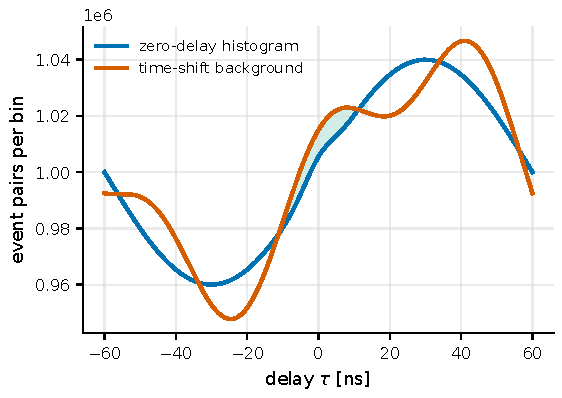
\includegraphics[width=0.72\linewidth]{figures/generated/chapter_07/ch07_time_shift_background.pdf}
\caption{时移背景估计的结构。蓝线是零延迟附近的事件对直方图，橙线是把一路整体平移到非物理延迟后得到的随机符合背景，绿色区域是中央峰相对时移背景的超额。这个方法能保留慢变率、坏时间和背景结构，但平移量必须远大于仪器响应宽度和天体相关宽度。}
\label{fig:e14-timeshift}
\end{figure}

\paragraph{连续波形的版本：Pearson 相关}

若硬件给的不是离散事件、而是连续采样的电压/电流波形（MAGIC-SII 就是），基本量改成\textbf{Pearson 相关系数}：
\begin{equation}
  \rho_{ab}(\tau_k)
  =\frac{\sum_n\big[x_a(t_n)-\bar x_a\big]\big[x_b(t_n+\tau_k)-\bar x_b\big]}
        {\sqrt{\sum_n\big[x_a(t_n)-\bar x_a\big]^2\;\sum_n\big[x_b(t_n)-\bar x_b\big]^2}} .
  \label{eq:e14-pearson}
\end{equation}
\begin{formulaexplain}
\(\rho_{ab}\) 衡量两路去均值波形的同步涨落；\(x_a,x_b\) 是采样电压/电流，\(\bar x\) 是各自平均。分母做归一，让 \(\rho\in[-1,1]\)；但它还混着恒星、夜天光、电子噪声，需再定标才成 \(|V|^2\)。
\end{formulaexplain}
Pearson 相关在硬件里实时算很方便（就是去均值、相乘、累加），但它测到的是三种涨落的混合，必须用直流电流、背景像素、零基线标定，才能转成物理的平方可见度 \(|V|^2\) \citep{2024MNRAS.529.4387A}。最后一个工程细节：格宽 \(\Delta\tau\) 要和相关峰宽、时间戳量化一起选——太宽会把峰高稀释掉，太窄则相邻格强相关、计算量白涨；VERITAS-SII 的相关 lag 间隔取 4 ns、峰宽也约 4 ns，而几十皮秒的 TDC 可以把格切得更细，前提是几何延迟、仪器响应、时钟残差都同等精度 \citep{2020NatAs...4.1164A,2020RScI...91a3108W,2009A&A...508..531N}。

\section{相关器如何在一夜之内算完}
\label{sec:e14-scaling}

现在面对一个纯工程问题：式 \eqref{eq:e14-paircount} 那个双重求和，真的能算完吗？

\textbf{最朴素的逐对法}。两路各有 \(N_a,N_b\) 个事件，全量比较就是 \(N_aN_b\) 次差分；若是同一路自相关，则是 \(N(N-1)/2\) 对。取 \(N_a=N_b=10^{9}\)，那是 \(10^{18}\) 次差分——即便每秒十亿次（\(10^{9}\,\mathrm{s^{-1}}\)，单核大致的现实速率），也要 \(10^{18}/10^{9}=10^{9}\,\mathrm s\approx30\) 年。逐对法只配用来做小样本教学检验。

\textbf{排序窗口法}。真相关峰只在很窄的延迟窗内，没必要比较相隔几秒的事件对。把两路都按时间排序，只在 \(|t_{j,b}-t_{i,a}|\le W\) 的滑动窗内找对，需检查的候选对数约为
\begin{equation}
  N_{\rm pair}^{\rm win}\simeq 2W\,R_b\,N_a .
  \label{eq:e14-window}
\end{equation}
\begin{formulaexplain}
\(N_{\rm pair}^{\rm win}\) 是窗口法要检查的候选对数；\(W\)（单位 s）是最大延迟窗半宽，\(R_b\) 是第二路率，\(N_a\) 是第一路事件数。有限窗把复杂度从 \(N^2\) 拉回近线性。
\end{formulaexplain}
代入 \(W=100\,\mathrm{ns}\)、\(R_b=10^{6}\,\mathrm{s^{-1}}\)、\(N_a=10^{9}\)：候选对约 \(2\times10^{-7}\times10^{6}\times10^{9}=2\times10^{8}\)，比全量双循环少了整整十个数量级，一台工作站几分钟就能扫完。而且排序窗口法保留每个事件的全部标签（波长、偏振），方便事后重新筛选。

\textbf{FFT 相关：XF 与 FX 两种排法}。若已经把事件或波形放进均匀时间格，可用快速傅里叶变换把时域互相关变成频域相乘：
\begin{equation}
  c_{ab}[k]
  =\mathcal F^{-1}\!\Big[\mathcal F\{x_a[n]\}^{*}\,\mathcal F\{x_b[n]\}\Big]_k .
  \label{eq:e14-fft}
\end{equation}
\begin{formulaexplain}
\(c_{ab}[k]\) 是离散互相关；\(\mathcal F,\mathcal F^{-1}\) 是离散傅里叶正/反变换，星号是复共轭。它把逐格相乘累加（\(O(N_{\rm bin}^2)\)）换成频域一次相乘（\(O(N_{\rm bin}\log N_{\rm bin})\)），\(N_{\rm bin}\) 是均匀时间格的格数（这里另起一个记号，别和后面误差预算里表示时移背景个数的 \(M\) 混淆）。
\end{formulaexplain}
这里就出现射电阵列里熟悉的两种相关器分工：\textbf{XF} 型先做互相关（correlate，得到延迟域的 \(c_{ab}[k]\)）再傅里叶变换成谱；\textbf{FX} 型反过来，先对每路各做一次 FFT（Fourier），再在每个频道上把各路两两相乘（cross-multiply）。为什么台站一多就偏爱 FX？因为 FFT 是"每路一次"的开销，随台站数 \(N_{\rm tel}\) 线性增长；而两两相乘那步无论哪种排法都是 \(O(N_{\rm tel}^{2})\)、躲不掉。台站少时（今天的强度干涉阵列往往只有 2–4 台，配对数 \(N(N-1)/2\) 很小），瓶颈根本不在配对数，而在\textbf{每对要吞的时间样本数}——这才是相关器真正的重活。

\begin{figure}[tbp]
\centering
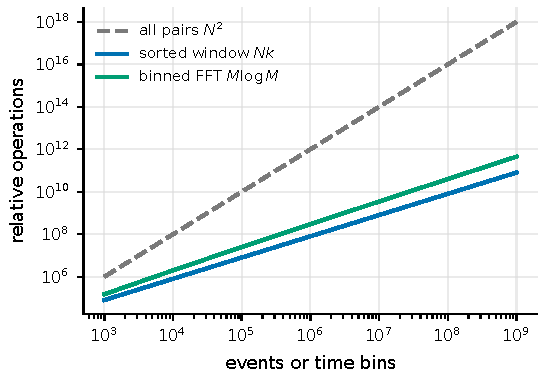
\includegraphics[width=0.72\linewidth]{figures/generated/chapter_07/ch07_correlator_scaling.pdf}
\caption{三类相关计算的操作数标度。全量逐对双循环随 \(N^2\) 疯长，只适合小样本或教学检验；排序窗口只比较有限延迟内的对，近似线性；均匀分箱后的 FFT 相关随 \(N_{\rm bin}\log N_{\rm bin}\) 增长，适合连续采样和实时监控。实际速度还受内存带宽、I/O、GPU/FPGA 数据排布和质量筛选左右。}
\label{fig:e14-scaling}
\end{figure}

\textbf{实时、无死时间的硬件相关}。VERITAS-SII 把连续 PMT 波形流到磁盘、再用 FPGA 离线相关；MAGIC-SII 则用 GPU 在观测当下实时算四通道所有配对相关 \citep{2020NatAs...4.1164A,2024MNRAS.529.4387A}。连续波形相关有一个单光子计数比不了的好处：它不靠"逐个光子触发—复位"，因此没有单光子探测器那种每次计数后的死时间盲区，能不间断地把整段涨落都算进相关里；这对信号只有 \(10^{-6}\)–\(10^{-4}\) 的强度干涉尤其重要，任何被丢掉的时间都是白扔的信噪比。多通道 TCSPC 则输出按时间排序的事件流，便于离线构造任意延迟和通道选择 \citep{2020RScI...91a3108W}。实时相关还能在观测中当场发现时钟跳变、电子串扰、云导致的通量突变——代价是通常只保存压缩后的相关产品。为长期归档，最好把原始事件/波形、标定事件、相关产品都留一份：FITS BINTABLE 适合事件归档，HDF5/Parquet 适合列式大数据，Astropy 帮着处理 FITS、时间和坐标元数据 \citep{2010A&A...524A..42P,2013A&A...558A..33A,2018AJ....156..123A}。

\section{误差为什么不是一串独立误差棒}
\label{sec:e14-cov}

到这里我们有了一条 \(\widehat g^{(2)}(\tau_k)\) 或一组 \(|V|^2\)。给每个点配一根 \(\sqrt N\) 误差棒、当作彼此独立，是初学者最常犯的错。先看理想情形下误差该有多大，再看真实数据为什么偏离它。

设信号窗计数 \(C_{ab,k}\) 是独立泊松量，背景由 \(M\) 个等权时移估计、\(\widehat B_{ab,k}=\frac1M\sum_{m=1}^{M}B_m\)，每个 \(B_m\) 是均值为 \(B\) 的独立泊松量。中央超额 \(X=C-\widehat B\) 的方差怎么算？泊松量方差等于均值，故 \(\operatorname{Var}(C)\approx C\)；背景平均后 \(\operatorname{Var}(\widehat B)=\frac1{M^2}\sum_m\operatorname{Var}(B_m)=\frac1{M^2}\,(M\,B)=B/M\)。两者独立、方差相加：
\begin{equation}
  \operatorname{Var}\!\big[\,C_{ab,k}-\widehat B_{ab,k}\,\big]
  \simeq C_{ab,k}+\frac{1}{M}\,B_{ab,k} .
  \label{eq:e14-excess-var}
\end{equation}
\begin{formulaexplain}
第一项 \(C_{ab,k}\) 是信号窗自身的泊松噪声，第二项 \(B_{ab,k}/M\) 是 \(M\) 个时移背景平均后的残余不确定度。\(M\) 越大，背景估得越稳。这是"事件独立、率稳定"理想下的误差预算。
\end{formulaexplain}
但式 \eqref{eq:e14-excess-var} 只在事件独立、时移背景互不重叠、率稳定时成立。真实数据里到处是"共享"：相邻延迟格共享同一批事件；多条基线共享同一台望远镜；多个波长通道共享同一片天气和同一路增益；多个模型点共享同一次零基线归一化。任何被共享的东西，都会让不同数据点的误差\textbf{相关}起来——误差矩阵不再是对角的。

于是要把全部相关产品当成一个向量、配一个协方差矩阵：
\begin{equation}
  \bm d=\big(\widehat{|V|^2}_1,\ \widehat{|V|^2}_2,\ \ldots,\ \widehat{|V|^2}_{N_d}\big),
  \qquad
  \Sigma_{ij}=\big\langle(d_i-\mu_i)(d_j-\mu_j)\big\rangle .
  \label{eq:e14-cov}
\end{equation}
\begin{formulaexplain}
\(\bm d\) 是相关产品数据向量，\(d_i\) 是第 \(i\) 个 \(|V|^2\) 点，\(\mu_i\) 是其均值；\(\Sigma_{ij}\) 是协方差矩阵，对角是各点方差，非对角记录"共享望远镜/背景/定标"造成的相关误差。
\end{formulaexplain}
\(\Sigma\) 从哪来？四条路子：解析误差传播（像式 \eqref{eq:e14-excess-var}）、时间块 bootstrap、jackknife（逐一剔除一台望远镜或一夜）、以及端到端注入仿真。时间块 bootstrap 是最实用的：把整夜数据切成许多时间块，块长要长于相关峰宽、电子噪声相关时间和指向/天气短时波动（夜级数据常取 10 s 到几分钟），随机有放回地重采样这些块、重算 \(|V|^2\)，块间的散布就直接给出协方差——顺带还检验了误差是否随积分时间以 \(T^{-1/2}\) 收敛。MAGIC-SII 就把电子带宽、光学带宽、直流读出增益、背景扣除、残余电子噪声都列成系统项，并通过朝极端方向摆动 \(|V|^2\) 数据点来估角直径的系统误差 \citep{2024MNRAS.529.4387A}。

\begin{figure}[tbp]
\centering
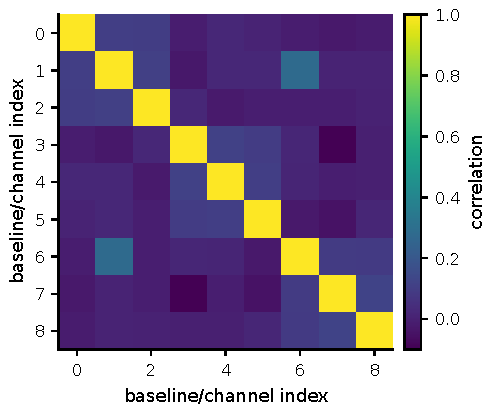
\includegraphics[width=0.66\linewidth]{figures/generated/chapter_07/ch07_covariance_matrix.pdf}
\caption{多基线/多通道结果的协方差矩阵示意。对角是单点方差，靠近对角的方块来自同一时间段或同一望远镜共享的噪声，远离对角线的结构可能来自共同背景估计、零基线归一化或电子串扰。若拟合只用对角误差，就会把"有效独立信息量"高估，误差棒假性变小。}
\label{fig:e14-cov}
\end{figure}

最后一句忠告：所有空检验（null test）都要用与主分析\textbf{同一套}选择函数和权重。常用空检验包括——把一路平移到非物理延迟、交换正负几何延迟、用两个本不该相关的偏振或波长通道、拿目标外天空当背景、把望远镜对分成不同时间块、逐一剔除某台望远镜或某夜、在真实事件表里注入已知相关峰看能否无偏恢复。若主信号只在某个阈值下冒头，一挪阈值、错延迟或做 jackknife 就消失，那它更可能是管线选择或仪器状态的产物，而不是天体相关。

\section{白噪声会沉降，系统误差是天花板}
\label{sec:e14-floor}

第 \ref{chap:e12} 章用 Fisher 信息回答过"数据里到底有多少信息"。这里把它接到时间上，讲清一个观测计划里最要命的分水岭：白噪声和系统误差，命运完全不同。

\textbf{白噪声（统计噪声）会沉降。}它来自光子的泊松涨落和电子的随机噪声，是一次次独立抽样。第 \ref{chap:e03} 章的结论：独立抽样越多，均值越稳，误差随有效光子数 \(N_{\rm eff}\) 以 \(N_{\rm eff}^{-1/2}\)、也就是随积分时间以 \(T^{-1/2}\) 下降。用 Fisher 语言说，独立数据点的信息是\textbf{相加}的，总信息随 \(N_{\rm eff}\) 线性增长，而 Cramér–Rao 下界给出的参数误差随信息平方根反比缩小——只要你肯积分，它就一直往下掉。

\textbf{系统误差（系统性偏差）不会沉降。}它来自定标不准、背景扣不干净、增益漂移、零基线不为零、电子带宽或光学带宽标定偏差这些\textbf{一致性偏移}。它们不是每次独立抽样，而是把每个数据点朝同一方向推同样一点点。再积分十倍时间，白噪声掉到 \(1/\sqrt{10}\)，可这个偏移纹丝不动——它成了一条水平的\textbf{地板}，误差再也下不去。

为什么这条地板对我们尤其致命？因为强度干涉的信号本就只有 \(10^{-6}\)–\(10^{-4}\) 那么微弱（回看式 \eqref{eq:e14-accidental} 下方那个 \(3.6\times10^4\) 对超额压在 \(3.6\times10^8\) 背景上的例子）。当你要测的超额只有百万分之一，那么背景定标只要有百万分之几的一致性偏差，就足以和信号同量级甚至淹没它。换句话说：微弱信号把系统误差的容忍度也压到了同样苛刻的 \(10^{-6}\) 级别，这正是本领域"系统项才是天花板"的根源。

把这句话数学化，就是把式 \eqref{eq:e14-cov} 的协方差喂进 Fisher 矩阵（推导见第 \ref{chap:e12} 章）：
\begin{equation}
  F_{\alpha\beta}
  =\frac{\partial\bm m^{T}}{\partial\theta_\alpha}\,\Sigma^{-1}\,\frac{\partial\bm m}{\partial\theta_\beta},
  \qquad
  \operatorname{Cov}(\theta_\alpha,\theta_\beta)\gtrsim(F^{-1})_{\alpha\beta} .
  \label{eq:e14-fisher}
\end{equation}
\begin{formulaexplain}
\(F_{\alpha\beta}\) 是 Fisher 信息矩阵：\(\partial\bm m/\partial\theta\) 是模型对参数的敏感度，\(\Sigma^{-1}\) 按协方差加权。其逆 \(F^{-1}\) 近似给出参数协方差下界。它是观测规划和高信噪比误差估计的主力工具。
\end{formulaexplain}
从这条式子能一眼读出两种标度。其一，\textbf{随光子数标度}：若 \(\Sigma\) 由独立光子统计主导，则 \(\Sigma^{-1}\propto N_{\rm eff}\)，\(F\propto N_{\rm eff}\)，参数误差 \(\propto N_{\rm eff}^{-1/2}\)——这就是白噪声的沉降。其二，\textbf{随基线标度}：Fisher 信息对相互独立的 \(uv\) 点是相加的，\(F=\sum_{\text{基线}}\)（各基线一项），所以多加一条基线就多一份信息。但一条基线值不值，取决于它落在模型 \(|V|^2\) 对参数最敏感、也就是 \(\partial\bm m/\partial\theta\) 最大的地方：对测角直径，最有价值的基线落在可见度曲线第一个零点附近（见第 \ref{chap:e10}、第 \ref{chap:e11} 章的 \(uv\) 覆盖讨论），落在 \(|V|^2\approx1\) 的短基线上则几乎不带角直径信息。可一旦 \(\Sigma\) 里出现那条不随时间下降的系统地板，\(\Sigma^{-1}\) 就饱和，再多光子、再长积分，\(F\) 也不再增长——误差趋于地板而止步。

\begin{figure}[tbp]
\centering
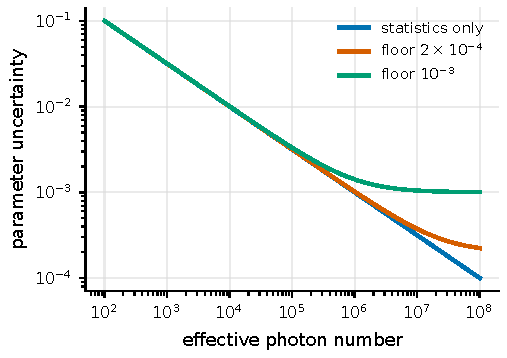
\includegraphics[width=0.70\linewidth]{figures/generated/chapter_07/ch07_fisher_scaling.pdf}
\caption{参数误差随有效光子数的标度。蓝线是纯统计的 \(N_{\rm eff}^{-1/2}\) 沉降；橙、绿线加入不同高度的系统地板后，长时间积分不再改善最终误差。观测计划必须把积分时间、目标亮度、基线覆盖、系统定标放进同一本误差预算里——这正是第 \ref{chap:e15} 章的主题。}
\label{fig:e14-fisher}
\end{figure}

最后提醒：Fisher 矩阵是似然峰附近的局部二次近似，只在高信噪比、后验近高斯时可靠。遇到多峰后验、非线性退化或参数贴边界，就得换 MCMC 或 nested sampling \citep{1925PCPS...22..700F,2013PASP..125..306F,2009MNRAS.398.1601F}。

\section{从相关产品到物理参数}
\label{sec:e14-fit}

有了带协方差的相关产品，最后一步是把物理参数拟合出来。先写\textbf{模型向量}：把角直径、双星分离、亮度比、环半径或喷流参数，映射成各个 \(uv\) 点、各个波长上的平方可见度：
\begin{equation}
  \bm m(\bm\theta)
  =\Big[\,|V(\bm u_1,\lambda_1\mid\bm\theta)|^2,\ \ldots,\ |V(\bm u_{N_d},\lambda_{N_d}\mid\bm\theta)|^2\,\Big] .
  \label{eq:e14-model}
\end{equation}
\begin{formulaexplain}
\(\bm m(\bm\theta)\) 是物理模型预言的数据向量，每项是空间频率 \(\bm u_i\)、波长 \(\lambda_i\) 处的 \(|V|^2\)。它把角直径、双星、结构等参数翻译成可与 \(\bm d\) 直接比较的观测量。
\end{formulaexplain}
这里 \(\bm u=\bm B_\perp/\lambda\) 是空间频率（以波长为单位的投影基线，见第 \ref{chap:e10} 章的 van Cittert–Zernike 定理）。若数据向量 \(\bm d\) 已近似高斯，似然就是带协方差加权的残差：
\begin{equation}
  -2\ln L
  =\big[\bm d-\bm m(\bm\theta)\big]^{T}\Sigma^{-1}\big[\bm d-\bm m(\bm\theta)\big]
   +\ln|\Sigma|+\text{const} .
  \label{eq:e14-gauss}
\end{equation}
\begin{formulaexplain}
\(\bm d-\bm m\) 是数据与模型残差，\(\Sigma^{-1}\) 按协方差加权（相关的点不重复计信息），\(\ln|\Sigma|\) 是归一化项。这是带相关误差的数据产品最常用的高斯似然，最小化它就得到最优参数。
\end{formulaexplain}
注意 \(\Sigma^{-1}\) 那一步正是第 \ref{sec:e14-cov} 节的回报：用完整协方差而不是对角误差，才不会把相关点当成互相独立、把信息量算多。要是直接拟合原始低计数延迟格，就别用高斯，回到式 \eqref{eq:e14-binned-poisson} 的泊松似然。VERITAS-SII 用均匀圆盘和临边昏暗模型拟合 \(|g^{(1)}|^2\) 随投影基线的变化；MAGIC-SII 把 Pearson 相关经通量和背景定标转成 \(|V|^2\) 后拟合角直径与系统误差 \citep{2020NatAs...4.1164A,2024MNRAS.529.4387A,1967MNRAS.137..375H}。

当后验可能多峰、或需要外部先验时，就写成\textbf{贝叶斯后验}：
\begin{equation}
  p(\bm\theta\mid\mathcal D,M)=\frac{L(\mathcal D\mid\bm\theta,M)\,\pi(\bm\theta\mid M)}{Z_M},
  \qquad
  Z_M=\int L\,\pi\,d\bm\theta .
  \label{eq:e14-posterior}
\end{equation}
\begin{formulaexplain}
\(p(\bm\theta\mid\mathcal D,M)\) 是模型 \(M\) 下的参数后验，\(L\) 是似然，\(\pi\) 是先验，\(Z_M\) 是模型证据（归一常数，也用来比较模型）。它把数据约束和外部物理知识合成完整的不确定度。
\end{formulaexplain}
先验 \(\pi\) 可以装距离、光谱型、已知角直径、双星轨道、爆发时间或物理边界——一定要写清楚，因为强度干涉常只测 \(|V|^2\)、缺相位，会让镜像、亮度比、位置角出现退化，是先验帮忙把退化按住。采样上，emcee 适合中等维度后验，MultiNest 适合多峰后验和证据估计 \citep{2013PASP..125..306F,2009MNRAS.398.1601F}；但采样器替代不了物理检查：链的自相关时间、接受率、先验体积、以及"注入已知信号能否无偏恢复"都要一并报告 \citep{1992ApJ...398..146G}。这样一条从事件表到带误差参数的链路才算闭合，第 \ref{chap:e15} 章会把它放进完整的观测设计与可行性评估。

\section{本章要点}
\label{sec:e14-summary}

\begin{itemize}
  \item \textbf{先建模型，再算估计量。}事件表要先写成选择函数式 \eqref{eq:e14-selection} 和泊松似然式 \eqref{eq:e14-point-likelihood}/\eqref{eq:e14-binned-poisson}；点过程似然由"无限窄分箱取极限"自然得到，能保留分箱后丢失的时间信息。
  \item \textbf{相关峰是巨大背景上的微弱超额。}延迟直方图式 \eqref{eq:e14-paircount} 要除以随机符合背景式 \eqref{eq:e14-accidental} 才有意义；真实信号只占背景的 \(10^{-6}\)–\(10^{-4}\)，这从根本上决定了积分时间和定标精度的要求。
  \item \textbf{算得完靠算法，不靠蛮力。}逐对 \(N^2\)/\(N(N-1)/2\) 只配教学；排序窗口式 \eqref{eq:e14-window} 近线性，FFT（XF/FX）随 \(N_{\rm bin}\log N_{\rm bin}\)；台站少时瓶颈在每对吞的时间样本数，GPU/FPGA 实时、无死时间相关把整段涨落都算进去。
  \item \textbf{误差不是独立误差棒。}共享望远镜、背景、定标会让协方差式 \eqref{eq:e14-cov} 出现非对角项；用时间块 bootstrap/jackknife/注入仿真估 \(\Sigma\)，拟合式 \eqref{eq:e14-gauss} 必须用完整 \(\Sigma^{-1}\)。
  \item \textbf{白噪声沉降，系统误差是天花板。}统计误差随 \(N_{\rm eff}^{-1/2}\)、\(T^{-1/2}\) 下降，Fisher 信息随光子数线性、对独立基线相加；但一致性偏移形成不随积分下降的地板，微弱信号把系统容忍度压到同样苛刻的量级。
\end{itemize}

\medskip
\noindent\textbf{想一想。}
(1) 若把延迟格宽 \(\Delta\tau\) 缩小一半，随机符合背景 \(B_{ab,k}\) 和信号超额各怎样变化，最终信噪比是否改善？
(2) 你有 4 台望远镜，为什么"配对数只有 6"并不意味着相关器很轻松？瓶颈在哪个量上？
(3) 一个团队积分时间翻了 10 倍，误差棒却几乎没变小。用本章语言，最可能的诊断是什么？该做哪些空检验去确认？
